\chapter{System modeling}
In this chapter, we focus on describing the System designs. We will start with the general architecture of our system, and then continue to the Intent specification and the Conversation flow for the Chat System. Next, we will describe the system design at the level of classes and interfaces to show their features, constraints and relationships. Our database design and mock-up design will also be reported.
\section{General Architecture}
\begin{figure}[H]
    \centering
    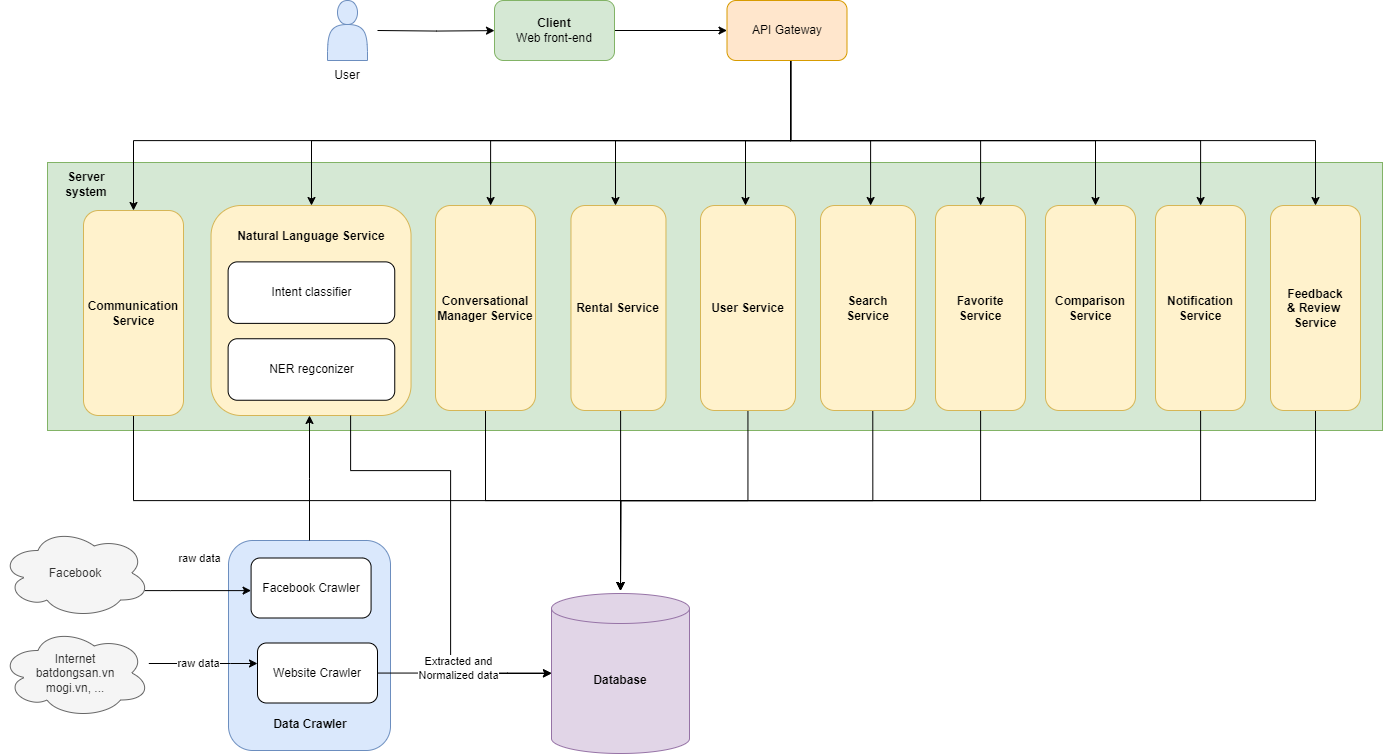
\includegraphics[width=\textwidth]{Images/System_architecture.png}
    \caption{System design: system architecture}
    \label{fig:sys-architect}
\end{figure}
Regarding the system's architectural approach, we are considering a combination of client-server architecture and micro-services in the server. The client-side, which provides the user interface to interact with the System, can be accessed by the User like a web application on a personal computer. On the server side, we break the system down into multiple modular and independent services. The server of the system contains 5 Microservices:
\begin{itemize}
    \item \textbf{Natural Language Service:} classify the intent and recognize the Name entities to catch the criteria in the User's message.
    \item \textbf{Conversational Manager Service:} control the conversational flow and generates a response to the User.
    \item \textbf{Rental Service:} manage the rental properties.
    \item \textbf{User Service:} manage user's account.
    \item \textbf{Search Service:} responsible for the rental searching request from the User.
    \item \textbf{Favorite Service:} provides functionality for users to save, organize, and interact with their favorite rental within the system.
    \item \textbf{Comparison Service:} responsible for the comparison 2 rental feature 
    \item \textbf{Notification Service:} Manage and deliver notifications according to the event. The events could be new messages incoming, updates on favorite rentals, ...
    \item \textbf{Communication Service:} responsible for communication and chatting between users.
\end{itemize}

Furthermore, we also decided to implement an API Gateway. The API Gateway is like an intermediary, functioning as the only entry point to our microservices system. It takes in requests from the client, performs necessary modifications, authenticates them, and then directs these requests to specific APIs within the backend services.

In addition, we decided to use a shared database for our system in this phase. The purpose of using a shared Database is to simplify schema management and to make data retrieval more efficient since all relevant information is stored in a centralized database, services can access the necessary data without the need for complex communication protocols.

\section{Intent specification}
We define the intents of our system as follows:

\subsection{Search intent}
\textbf{Description}: The intent Search is triggered when the user wants to search for the accommodations. The user can provide the location, price, area, or other criteria to search for the accommodations. 

\noindent \textbf{Example}: Some examples of the Search intent are shown below:
\begin{itemize}
    \item "Tôi muốn tìm phòng trọ quận 10, gần đại học Bách Khoa" (I want to find a room in district 10, near Bach Khoa University)
    \item "Tôi muốn tìm phòng trọ giá dưới 2 triệu" (I want to find a room with the price under 2 million VND)
\end{itemize} 

\noindent \textbf{Expected response}: The chatbot will return a list of rental posts that match the user's preferences.

\subsection{Post intent}
\textbf{Description}: The Post intent is triggered when the landlord wants to post their room for rent. Same with the Search intent, the user can provide some additional information such as the location, price, area, or other criteria. 

\noindent \textbf{Example} Some examples of the Post intent are:
\begin{itemize}
    \item "Tôi có phòng trọ trống tại quận 10, cần cho thuê với giá 2 triệu" (I have a room for rent in district 10 with the price of 2 million VND)
    \item "Tôi muốn đăng phòng trọ ở quận 10, gần đại học Bách Khoa" (I want to post a room in district 10, near Bach Khoa University)
\end{itemize}

\noindent \textbf{Expected response}: The chatbot will ask the landlord to provide more required information about the room such as the price, location, and area, ... Then the chatbot will post the room on the website.

\subsection{Provide information intent}
\textbf{Description}: The Provide information intent is triggered when the user answers the chatbot's question. 

\noindent \textbf{Example}: Some examples of the Provide information intent are:
\begin{itemize}
    \item Chatbot: "Bạn cần tìm phòng trọ ở đâu?" (Where do you want to find a room?). User: "Quận 10" (District 10)
    \item Chatbot: "Bạn cần tìm phòng trọ giá khoảng bao nhiêu?" (What is your budget?). User: "Dưới 2 triệu" (Under 2 million)
\end{itemize}

\noindent \textbf{Expected response}: The chatbot will store the information provided by the user for later actions.

\subsection{Other intents}
Besides the main intents above, we also define some other intents such as Greeting, Confirm, Reject, and Fallback that support the process of getting information from the user. 

{\renewcommand{\arraystretch}{1.75}%
\begin{table}[ht]
    \centering
    \begin{tabular}{|l|l|}
        \hline
        \textbf{Intent} & \textbf{Description} \\ \hline
        Greeting & Users want to greet the chatbot and start the conversation. \\ \hline
        Confirm & Users confirm the information that the chatbot responds to. \\ \hline
        Reject & Users reject the information that the chatbot responds to. \\ \hline
        Fallback & Triggered when the user's message does not match any of the intents above.  \\ \hline
    \end{tabular}
\end{table}}

\section{Entities Specifications}
In this section, we define the entities of our system in Figure \ref{fig:entities} and the specifications in Table \ref{tab:entities-specifications}.

\begin{figure}[ht]
    \centering
    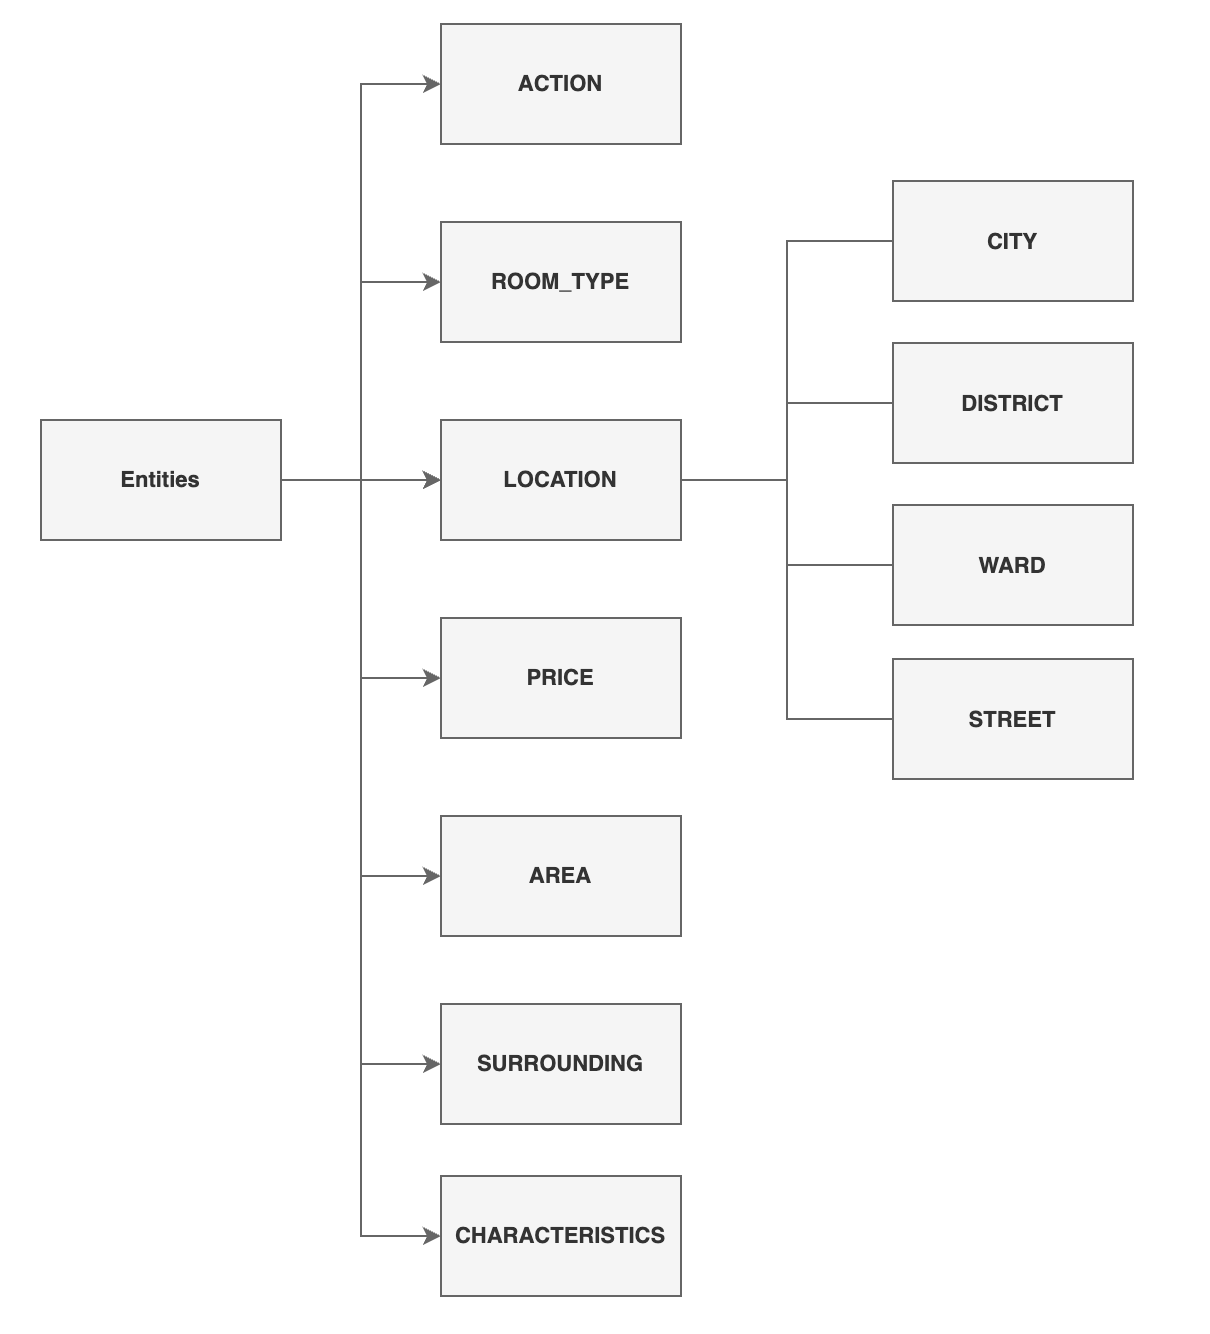
\includegraphics[width=0.8\textwidth]{../Images/7.System_Modeling/entities.png}
    \caption{Entities of the system}
    \label{fig:entities}
\end{figure}

{\renewcommand{\arraystretch}{1.75}%
\begin{table}[ht]
    \centering
    \begin{tabular}{|l|l|}
        \hline
        \textbf{Entites} & \textbf{Description} \\ \hline
        ACTION & The action that users want. Ex: tìm phòng (search) or cho thuê phòng (post). \\ \hline
        ROOM\_TYPE & The type of the room. Ex: phòng trọ (room for rent), chung cư (apartment),... \\ \hline
        CITY & The city name where the room is located. \\ \hline
        DISTRICT & The district name. Ex: quận 10 (district 10) \\ \hline
        WARD & The ward name. Ex: phường 14 (ward 14) \\ \hline
        STREET & The street name. Ex: đường Lý Thường Kiệt (Ly Thuong Kiet street)\\ \hline
        PRICE & The price of the room. Ex: 2 triệu, 2tr (2 million VND) \\ \hline
        AREA & The area of the room. Ex: 20m2, 20 mét vuông (20 square meters) \\ \hline
        SURROUNDING & The surrounding of the room (university, hospital,...)\\ \hline
        CHARACTERISTICS & The characteristics of the room. Ex: yên tĩnh, có chỗ để xe (has parking lot) \\ \hline

    \end{tabular}
    \caption{Entities specifications}
    \label{tab:entities-specifications}
\end{table}}
\clearpage

\section{Conversational Flow}

We have defined 2 main conversational flows for our system. The first flow is for the user to search for rental posts. The second flow is for the landlord to post their room for rent. The system conversational flow is shown in Figure \ref{fig:conversational-flow}.

\begin{figure}[ht]
    \centering
    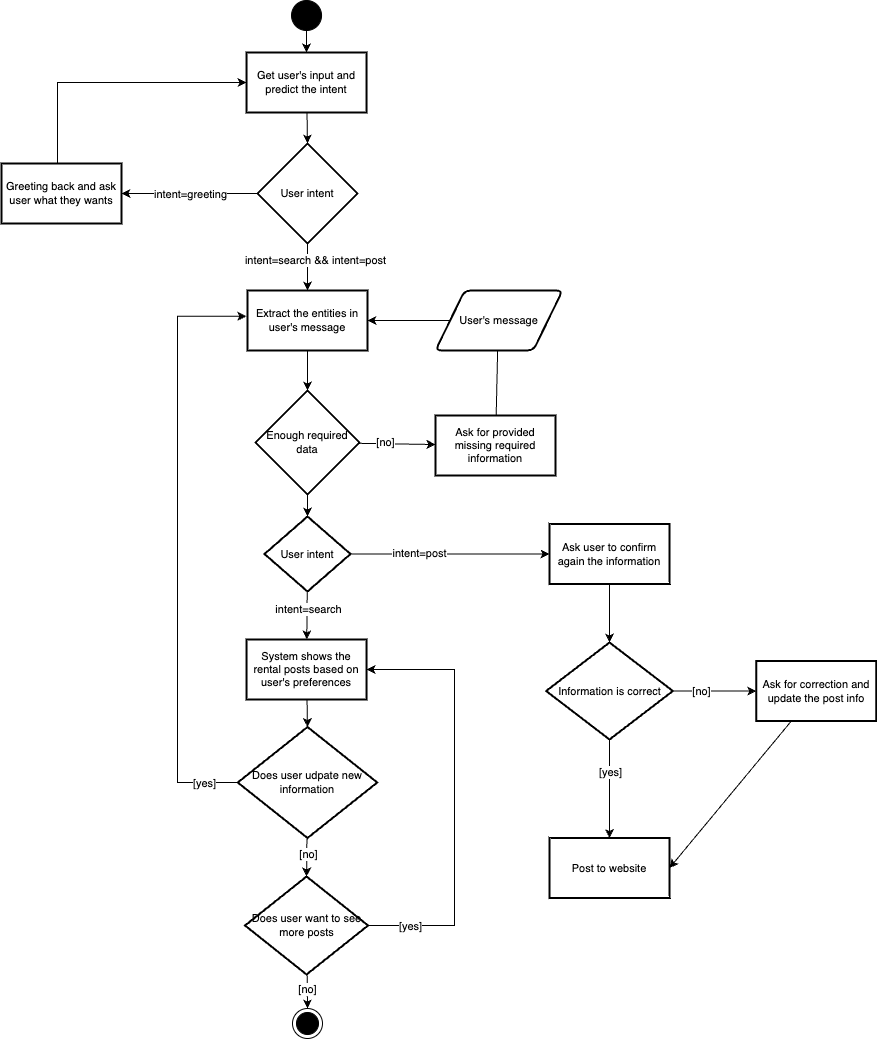
\includegraphics[width=0.8\textwidth]{../Images/7.System_Modeling/conversational_flow.png}
    \caption{The system conversational flow}
    \label{fig:conversational-flow}
\end{figure}

\section{Intent Classification Model}
\label{sec:intent-classification-model}
To implement the Intent Classification Model, we choose to follow the BERT feature-based approach. We use PhoBERT as the pre-trained language model to create word embedding vectors for the input. After that, the word embedding is fed into a fully connected neural network with the softmax layer to classify the intent. The model architecture is shown in Figure

\begin{figure}[ht]
    \centering
    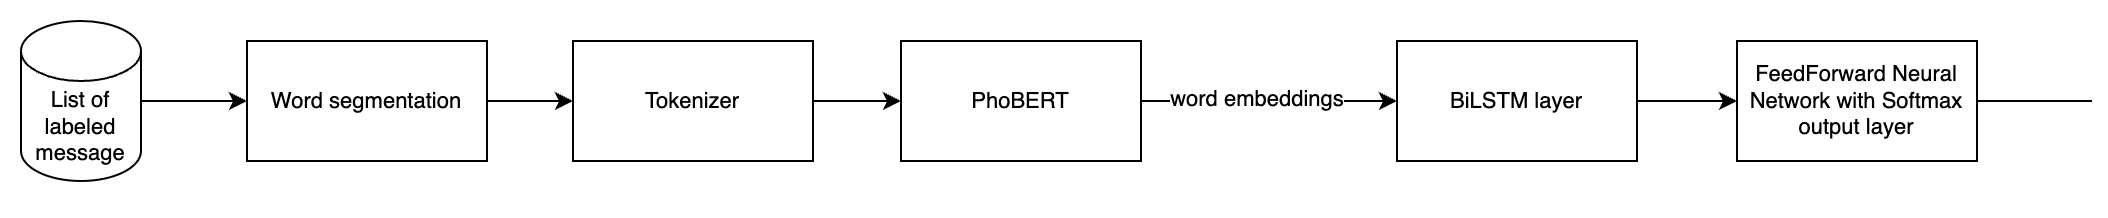
\includegraphics[width=\textwidth]{../Images/7.System_Modeling/intent_classifier_architecture.png}
    \caption{The architecture of Intent Classification Model}
    \label{fig:intent-classification-model}
\end{figure}

PhoBERT is trained on a large corpus of the Vietnamese language, so it can help our model have the general knowledge about the Vietnamese knowledge. Then we train the BiLSTM layer with the Fully Connected layer on the intent classification dataset, which allows the model to get the domain-specific knowledge and learn the pattern for the intent classification task. Our system has a total of 7 intents, so the output of the softmax layer is a vector of 7 elements. The element with the highest value is the predicted intent. 

\section{Named Entity Recognition Model}
We continue to use the PhoBERT feature-based approach for the Named Entity Recognition Model. The model architecture is shown in Figure \ref{fig:ner-model}.

\begin{figure}[ht]
    \centering
    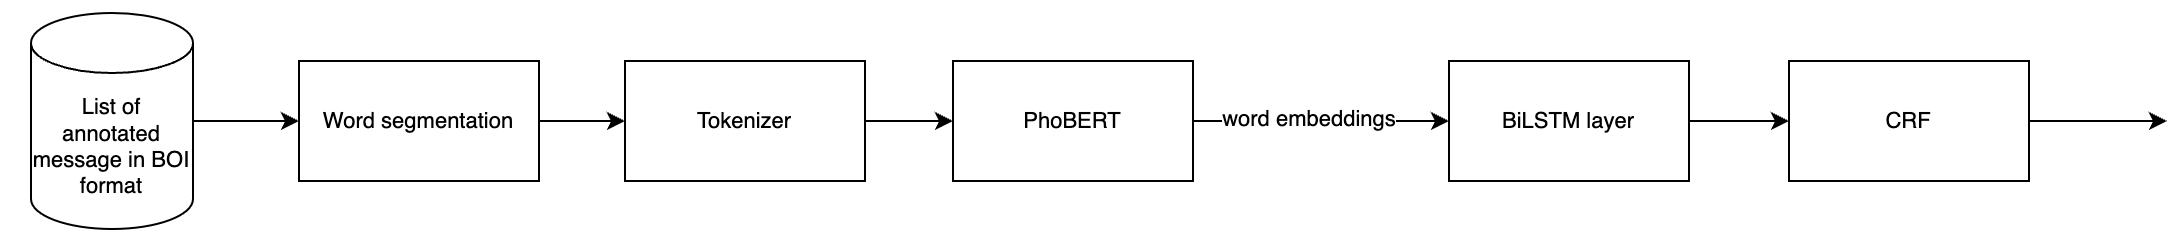
\includegraphics[width=\textwidth]{../Images/7.System_Modeling/ner_architecture.png}
    \caption{The architecture of Named Entity Recognition Model}
    \label{fig:ner-model}
\end{figure}

To train the NER model, we need the annotated data in the BOI format that we mentioned in Chapter \ref{chap:theoretical-background}. We use the same pre-trained language model for both intent classification and NER. We can combine these two models after training independently. The output of the NER model is the value returned by the CRF (conditional random field) layer. The output of the CRF layer is the same length as the input. Each element of the output is the predicted tag for the corresponding word. The tag is one of the following values: B-ROOM\_TYPE, I-ROOM\_TYPE, B-CITY, I-CITY, B-DISTRICT, I-DISTRICT, B-WARD, I-WARD, B-STREET, I-STREET, B-PRICE, I-PRICE, B-AREA, I-AREA, B-SURROUNDING, I-SURROUNDING, B-CHARACTERISTICS, I-CHARACTERISTICS, O. The tag O means that the word is not an entity. 

% %%%%%% DATABASE DESIGN%%%%%%%%%%%%%%%%%%%%
\newpage
\section{Database Design}
The purpose of this Database is to store information about the user's account, rental post, favorite list, message, and notification. The database schema contains 12 entities, each entity is defined with its attributes. The list of entities and the relationship between these entities can be described using the ERD Diagram. 
\subsection{ERD Model}
\begin{figure}[H]
    \centering
    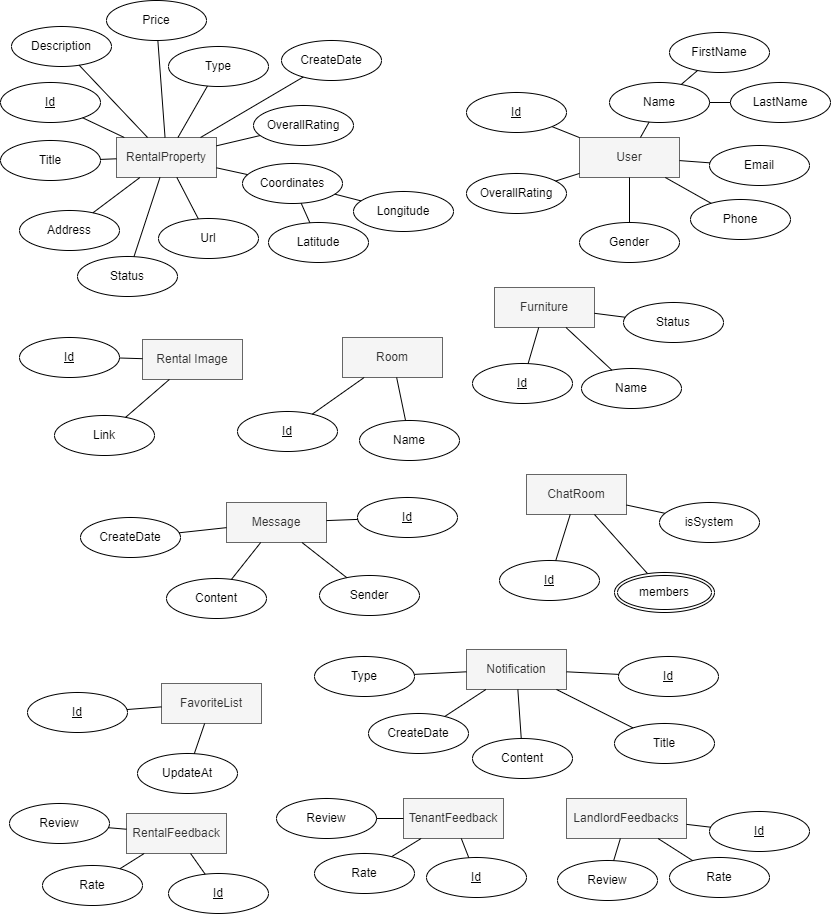
\includegraphics[width=0.85\textwidth]{Images/ERD.png}
    \caption{Database design: List of entities}
    \label{fig:DB-list-entities}
\end{figure}
The database should be able to store data related to the services according to the system architecture. Therefore, firstly we need to list out the entities with their attribute according to the requirement elicitation:
\begin{itemize}
    \item Listing and searching for rental properties
    \item Managing favorite list contains favorite rental
    \item Managing user accounts and profiles
    \item Sending and receiving messages through chats
    \item Sending and receiving notifications about rental properties and other system events
    \item Managing feedback about User and Rental
\end{itemize}

\begin{figure}[H]
    \centering
    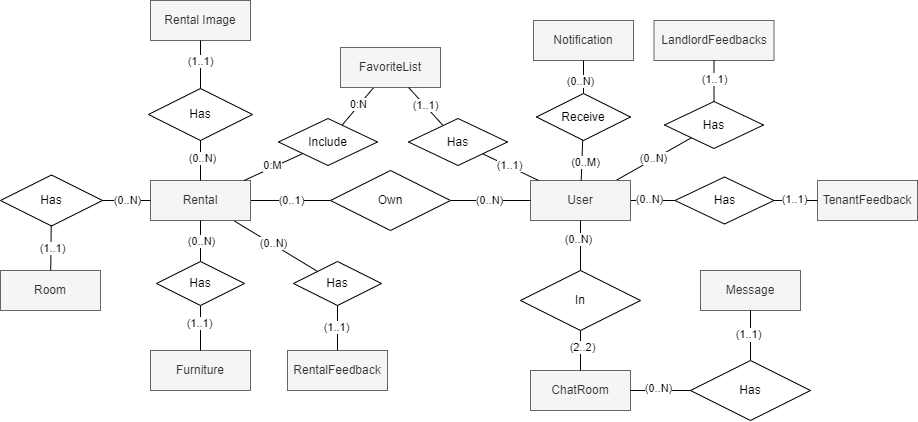
\includegraphics[width=\textwidth]{Images/ERD-Relationship.png}
    \caption{Database design: Entity - Relationship Diagram}
    \label{fig:erd-relationship}
\end{figure}
Next, we need to specify the relationships between these entities. The relationship can be described based on the specifications as follows:
\begin{itemize}
    \item A user can have zero or many rentals, and a rental can be associated with zero or many users (because some rentals might be crawled from the internet)
    \item A user can have zero or many feedback, while feedback must be associated with exactly one user. A user will have 2 view: user as the Tenant and user as the Landlord. By that reason, a User should have 2 type of feedback: Landlord feedback and Tenant feedback.
    \item A rental can have zero or many images, while each image must belong to exactly one rental.
    \item A rental can have zero or many room (bedrooms, living-rooms, bathrooms,...), while each room must belong to exactly one rental.
    \item A rental can have zero or many furniture (washing machine, stove, Wi-Fi, ...), while each furniture must belong to exactly one rental.
    \item A rental will also have zero or multiple feedback, and a rental feedback must also belongs to exactly one rental. 
    \item A user has one favorite rental list, and the list can contains zero or many rental.
    \item A User can receive notifications. Therefore, a user should be associated with multiple notification. Moreover, a notification can be published to multiple user.
    \item A user can join in multiple chat-room, while each chat-room should contains exactly 2 members (user - user or user - chat-bot).
    \item A chat-room also contains multiple messages, while a message must belongs to exactly 1 chat-room. 
\end{itemize}
\section{Mock-up}
\subsection{Tenant User Interface}
\subsection{Landlord User Interface}